

\documentclass[10pt, conference, compsocconf]{IEEEtran}

\ifCLASSINFOpdf

\else

\fi

\usepackage{hyperref}
\usepackage{amsmath}
\usepackage{amssymb}
\usepackage{hhline} % easy to manage table borders
\usepackage{colortbl} % colored cells in tables
\usepackage{multirow}
\usepackage{enumerate}
\usepackage{slashbox} % cell with slash inside
\usepackage{makeidx}  % allows index generation
\usepackage[utf8]{inputenc}
\usepackage{graphicx}

\newtheorem{definition}{Definition}
\newtheorem{example}{Example}

\def\sectionautorefname{Section}
\def\subsectionautorefname{Section}


% correct bad hyphenation here
\hyphenation{op-tical net-works semi-conduc-tor}


\begin{document}

% paper title
% can use linebreaks \\ within to get better formatting as desired
\title{Pharmer -- Towards Semantic Medical Prescriptions}
%\title{Pharmer: A platform for health care providers to use linked open data in e-prescriptions}


% author names and affiliations
% use a multiple column layout for up to two different
% affiliations

\author{\IEEEauthorblockN{Ali Khalili}
\IEEEauthorblockA{Institute of Informatics\\
University of Leipzig\\
Leipzig, Germany\\
khalili@informatik.uni-leipzig.de}
\and
\IEEEauthorblockN{Bita Sedaghati}
\IEEEauthorblockA{Institute of Pharmacy\\
University of Leipzig\\
Leipzig, Germany\\
bita.sedaghati@uni-leipzig.de}
}


% make the title area
\maketitle

\begin{abstract}
The abstract goes here. DO NOT USE SPECIAL CHARACTERS, SYMBOLS, OR MATH IN YOUR TITLE OR ABSTRACT.

\end{abstract}

\begin{IEEEkeywords}
component; formatting; style; styling;

\end{IEEEkeywords}


\IEEEpeerreviewmaketitle



\section{Introduction}
\label{intro}

As reported in MedicineNet\footnote{\url{http://www.medicinenet.com/}}, \emph{medication errors} are the most common type of medical errors in health care.
Errors such as improper dose of medicine, adverse drug interactions, food interactions, etc. often stem from invalid prescriptions and unawareness of the patients.
Electronic prescriptions which are recently gaining attention in the e-health domain, are one of the solutions proposed to solve these type of errors.
While even nowadays traditional paper prescriptions are commonly used, e-prescriptions offer several advantages.
In an e-prescription system, prescriber electronically sends an accurate, error-free and understandable prescription directly to a pharmacy from the point-of-care.
Reduction in medication error and decline in adverse drug events are more highlighted consequences of e-prescribing.

During the recent years, the adoption of e-prescriptions has been spreading rapidly.
To illustrate, the Australian government started launching of e-prescription from March 2007.
Using this system, the e-providers who effectively market themselves on the web will have a distinct advantage\cite{Ravichandran}.
A system called epSOS which performs the use of e-prescriptions all around Europe, is currently passing the extensive practical testing phase.
epSOS contains patient summery and an e-prescription service which allows access to the cross-border e-health services.
This service allows people in participating epSOS pilot countries, as tourists, business travellers, commuters or exchange students to take advantage of e-health services.
The e-Prescribing incentive program performed in US is another example in this area.
As a reporting program it uses a combination of incentive payments and payment adjustments to encourage electronic prescribing by eligible professionals.

One of the main challenges of using e-prescription systems is the heterogeneity of available information sources.
There exist already different sources of information addressing different aspects of pharmaceutical research.
Information about chemical, pharmacological and pharmaceutical drug data, clinical trials, approved prescription drugs, drugs activity against drug targets such as proteins, gene-disease-drug associations, adverse effects of marketed drugs, etc. are some examples of these diverse information.
Handling these information within current e-prescription systems without blurring the border of the existing pharmaceutical information islands is a cumbersome task.
On the other hand, \emph{Linked Open Data} as an effort to interlink and integrate these isolated sources of information is receiving more attention in the domain of medical and life sciences.
Combining the best practices from Linked Open Data together with e-prescription systems can provide an opportunity for patients, researchers as well as practitioners to collaborate together in a synergic way.

Semantic prescriptions as introduced in this paper are a proposed approach to utilize semantic web technologies in e-prescription systems.
As intelligent prescriptions, they can automatically handle the medical errors occurring in prescriptions and increase the awareness of the patients about the prescribed drugs and drug consumption in general.
Semantic prescriptions also enable the creation of more efficient and effective search approaches for drug discovery and consumption.
We created a tool called \emph{Pharmer} as a showcase application to facilitate the process of semantic prescription generation.

The remainder of this article is structured as follows:
\autoref{sec:lod}, \autoref{sec:sca} and \autoref{sec:epresc} provide a background on the basic concepts such as Linked Open Data, Semantic Content Authoring and E-prescriptions employed in this paper.


\section{Linked Open Data}
\label{sec:lod}
In computing, \emph{Linked Data} describes a method of publishing structured data so that it can be interlinked and become more useful.
It builds upon standard Web technologies such as HTTP and URIs, but rather than using them to serve web pages for human readers, it extends them to share information in a way that can be read automatically by computers.
This enables data from different sources to be connected and queried \cite{linkeddata}.

Tim Berners-Lee, the inventor of the Web and Linked Data initiator, suggested a 5 star deployment scheme for \emph{Linked Open Data}.

\begin{enumerate}
  \item  Make your stuff available on the Web (whatever format) under an open license
  \item  Make it available as structured data (e.g., Excel instead of image scan of a table)
  \item  Use non-proprietary formats (e.g., CSV instead of Excel)
  \item  Use URIs to identify things, so that people can point at your stuff
  \item  Link your data to other data to provide context
\end{enumerate}

\begin{figure}[tb]
	\centering
		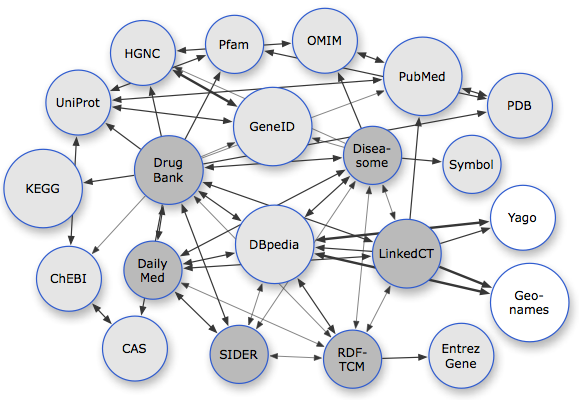
\includegraphics[width=1.0\columnwidth]{images/lod_cloud.png}
	\caption{Available datasets related to pharmaceutical research.}
	\label{fig:lod}
\end{figure}

Particularly in the areas of health care and life sciences with the wealth of available data, large scale integration projects like Bio2RDF\footnote{\url{http://bio2rdf.org/}}, Chem2Bio2RDF\footnote{\url{http://chem2bio2rdf.wikispaces.com/}}, and the W3C HCLS’s (Health Care and Life Sciences) Linked Open Drug Data (LODD)\footnote{\url{http://www.w3.org/wiki/HCLSIG/LODD}} have not only significantly contributed to the development of the Linked Open Data effort, but have also made social and technical contributions towards data integration, knowledge management, and knowledge discovery.

There are already many interesting information on pharmaceutical research available on the Web.
The sources of data range from drugs general information, interactions and impacts of the drugs on gene expression, through to the results of clinical trials (ss shown in \autoref{fig:lod}).
LODD\cite{lodrug} has surveyed publicly available data about drugs, created Linked Data representations of the data sets, and identified interesting scientific and business questions that can be answered once the data sets are connected.

One of the use cases of LODD datasets is authoring of \emph{Semantic Prescriptions} which are prescriptions enriched by linked open data.

\section{Semantic Content Authoring}
\label{sec:sca}
 A \emph{Semantic Document} is an intelligent document (with explicit semantic structure) which ``knows about" its own content so that it can be automatically processed in unforeseen ways.

Semantic documents facilitate a number of important aspects of information management~\cite{rdface}:
\begin{itemize}
	\item For \emph{search and retrieval} enriching documents with semantic representations helps to create more efficient and effective search interfaces, such as faceted search~\cite{tunkenlang2009faceted} or question answering~\cite{Lopez2011}.
		Ultimately, users are empowered to counter the increasing information overload and gain better access to relevant documents and answers related to their information needs.
	\item In \emph{information presentation} semantically enriched documents can be used to create more sophisticated ways of flexibly visualizing information, such as by means of semantic overlays as described in~\cite{Burel2009}.
	\item For \emph{information integration} semantically enriched documents can be used to provide unified views on heterogeneous data stored in different applications by creating composite applications such as semantic mashups~\cite{Ankolekar2007}.
	\item To realize \emph{personalization}, semantic documents provide customized and context-specific information which better fits user needs and will result in delivering customized applications such as personalized semantic portals~\cite{ecs2007}.
	\item For \emph{reusability} and \emph{interoperability} enriching documents with semantic representations (e.g. using the SKOS and Dublin Core vocabularies) facilitates exchanging content between disparate systems and enables building applications such as executable papers~\cite{Muller2011}. \\
\end{itemize}

These benefits, however, come at the cost of increased authoring effort~\cite{hasida2007,uren2006}.
\emph{Semantic Content Authoring} (SCA) is a tool-supported manual composition process aiming at the creation of semantic documents which are either:
\begin{itemize}
	\item fully semantic in the sense that their original data model uses a semantic knowledge representation formalism (such as RDF, RDF-Schema or OWL) or
	\item based on a non-semantic representation form (e.g. text or hypertext), which is enriched with semantic representations during the authoring process.\\
\end{itemize}

With an ontology and a user interface appropriate for the type of content, semantic authoring can be easier than traditional composition of content and the resulting content can be of higher quality~\cite{hasida2007}.
A \emph{Semantic Authoring User Interface} (SAUI) is a human accessible interface with capabilities for modifying and writing semantic documents.

Medical prescriptions are a good candidate to be enriched by semantic annotations.
Semantic prescriptions enable the traditionally written prescriptions to be utilized in novel ways as discussed above.
In the following sections, we first describe the e-prescriptions and then discuss how they can be enriched as semantic documents.

\section{e-prescriptions}
\label{sec:epresc}
E-health has evolved and emerged recently in many forms.
E-prescription is one of these forms and defined as a computer-generated prescription utilized by healthcare providers.
E-prescribing as it is commonly called, is the use of an automated data entry system to generate a prescription that is then transmitted through a special network to the pharmacy in such a way that the data goes directly into the pharmacy’s computer system.
It plays an important role in improving the quality of patient care.
For the prescriber, e-prescribing happens when a physician uses a computer or hand held device with software that allows him or her to—with a patient’s consent—electronically access information regarding a patient’s drug benefit coverage and medication history; electronically transmit the prescription to the patient’s choice of pharmacy; and, when the patient runs out of refills, his or her pharmacist can also electronically send a renewal request to the physician’s office for approval.

There are challenges that are solved by E-prescription systems.
Once writing a prescription it is very critical to consider drug interactions.
Drug interactions are divided to three categories namely \emph{food-drug}, \emph{drug-drug} and \emph{drug-plant} interactions.
Coadministration can either be synergistic or antagonistic which respectively increase or decrease the drugs effect.
The interactions may sometimes lead to change in the drug effect.
By applying E-prescription system, all types of drug interactions are prevented and the probability of errors in prescriptions are reduced to a great extend.
A E-prescription simply contains drug information and precautions which are necessary to be considered from patient's side.

Through electronic prescribing, all health care stakeholders including providers, patients, pharmacies, and payors benefits such as:
Payors/insurances: efficiency, prescription compliance and prevention of Adverse drug reactions.
Patients: Increased safety, efficiency and compliance, lowered co-pays
Providers: Increased efficiency, improved care, patient satisfaction and potential short and long-term incentives
Pharmacies: Increased efficiency, improved care, improved patient satisfaction

E-prescribing involves far more than an electronic connection. In order to see an increase in both quality and efficiency that can be attributed to e-prescribing, the system must be capable of performing key functions related to:
Medication selection/decision support capabilities (e.g., diagnosis-based medication menus, evidence based information, drug interaction checking, safety-alerts, formulary checking, prescription renewal, and dosage calculation)
Patient-specific information capabilities (e.g., current patient medication list, access to patient historical data, patient identification)
System integration capabilities (e.g., connection with various databases, connection with pharmacy and pharmacy benefit manager systems)
Educational capabilities (e.g., patient education, provider feedback)

The journey of an e-script begins when the patient and physician review history and discuss the current issue and treatment options. The patient’s up-to-date formulary and medication history is then presented to the provider at the point-of-care.
The physician then reviews clinical alerts, formulary, reference, prescription history and eligibility with the patient and selects therapy and verifies the patient’s preferred pharmacy.
Once the prescription is finalized, the e-script is generated and the physician routs it to the patient’s pharmacy of choice. The pharmacist fills the prescription and sends a fill notification to the physician.
The two-way connectivity provides for the transmission of new prescriptions, refill authorizations, and denials and change requests between the pharmacy and the provider’s office.

It is also evident by using the E-prescription, follow up of patient individuals is convenient.The next part of procedure occurs during the medication therapy and afterwards. The patient is supposed to report about his/her condition by returning to a physician or online contact.
The health care providers can access to the patient's profile and the transfer of these data can appropriately be done.
Besides, the data of medicines consumption and the connection between diagnosed disease and the treatment regimen is recorded.
Furthermore, patient's fate after the medication duration can be followed up by physicians and pharmacists.
The E-prescription information is  of crucial importance as an  informative source for researchers.
Many researchers investigate the aforementioned statistical data and combine them with the information received from the medicine producers (e.g. to compare the special drug consumption different  individual age ranges).


Another challenge points

 and needs to be more carefully investigated by health care providers.

1.Patient contact  physician in order to treat his  disease. By that he automatically enters To the online system.
2.Physician based on his diagnosis writes an  E-Rx in the system.
3.E-Rx immediately is sent to the patient’s chosen pharmacy and pharmacist verify the E-Rx and gives the medication to the patient.
4.Patient recieves the drugd from pharmacist and inquire about drugs.

\begin{figure}[tb]
	\centering
		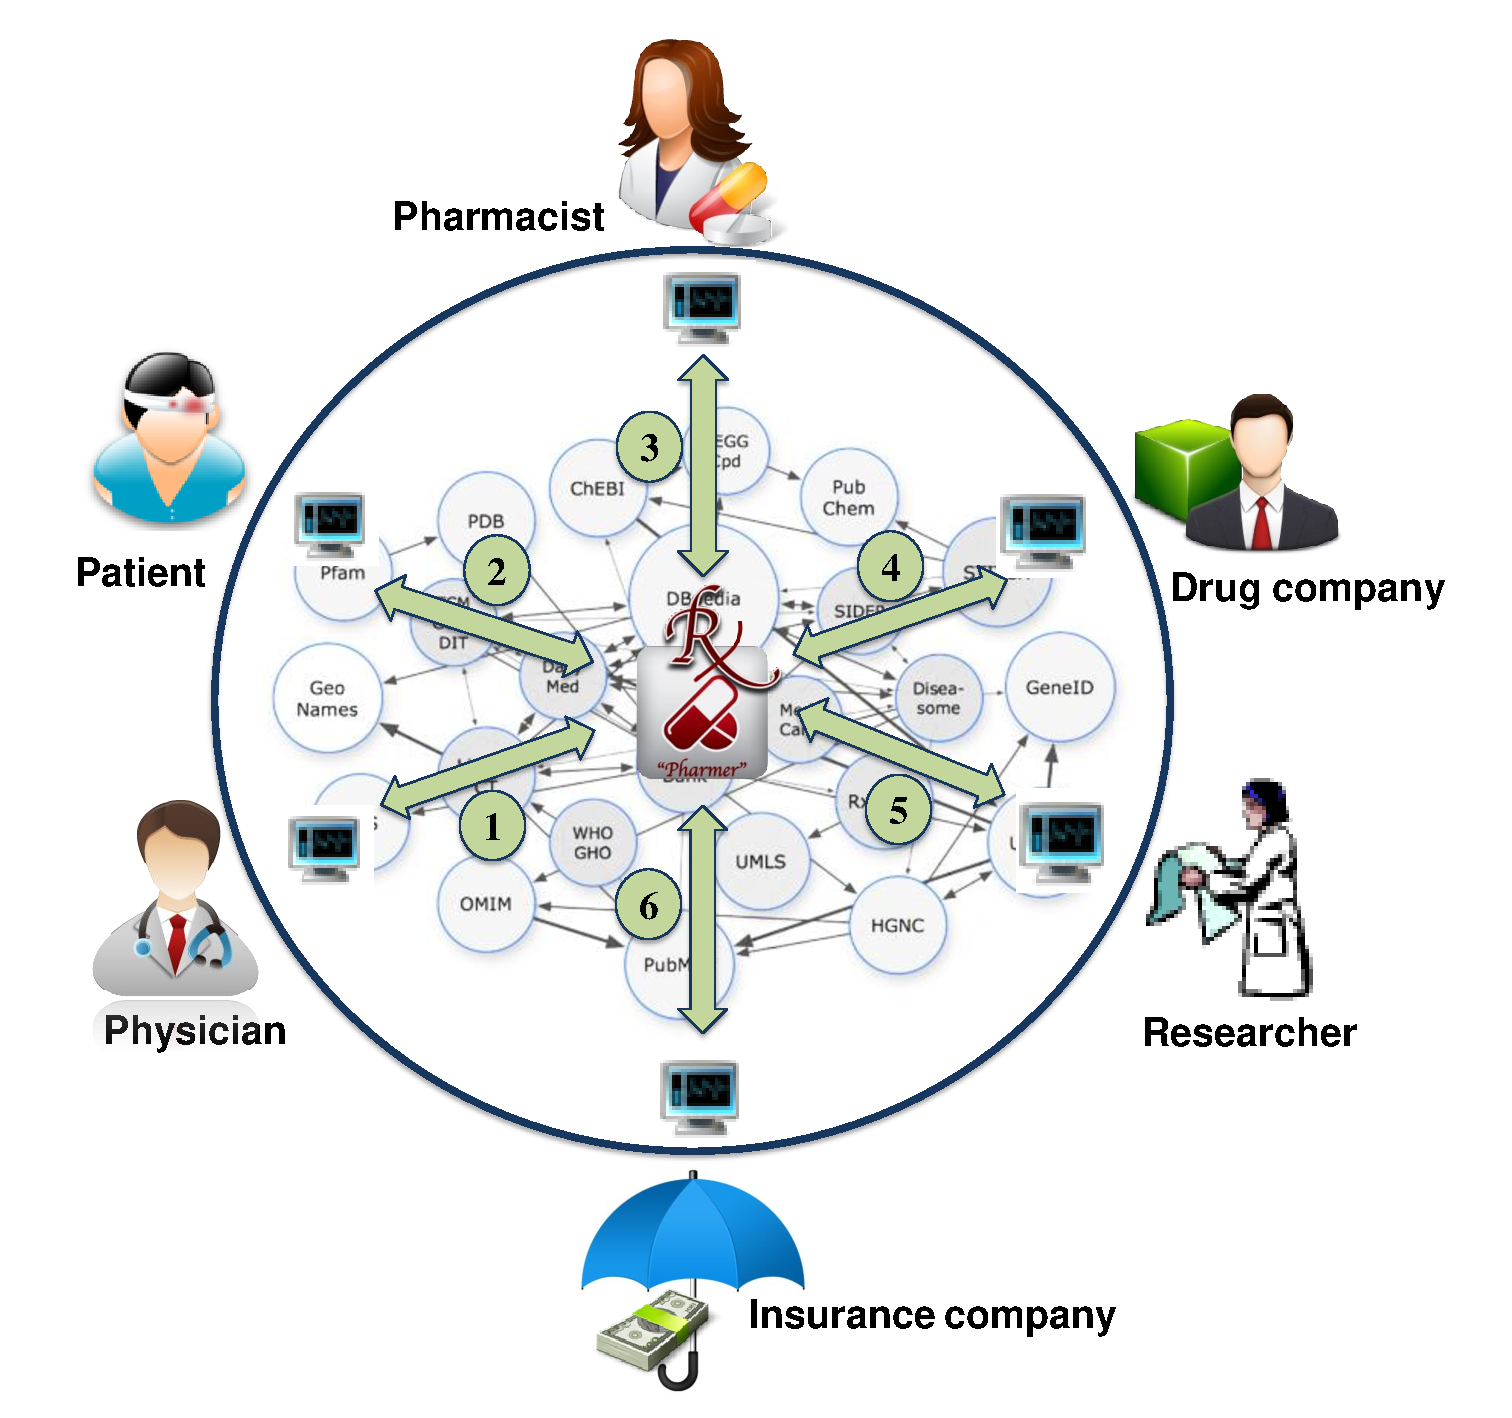
\includegraphics[width=1.0\columnwidth]{images/system.pdf}
	\caption{Pharmer ecosystem.}
	\label{fig:system}
\end{figure}

\section{Pharmer: Semantic Authoring of Medical Prescriptions}
\label{pharmer}


\subsection{Architecture}

The Pharmer system architecture is depicted in \autoref{fig:arch} and consists of three layers.

\begin{figure}[tb]
	\centering
		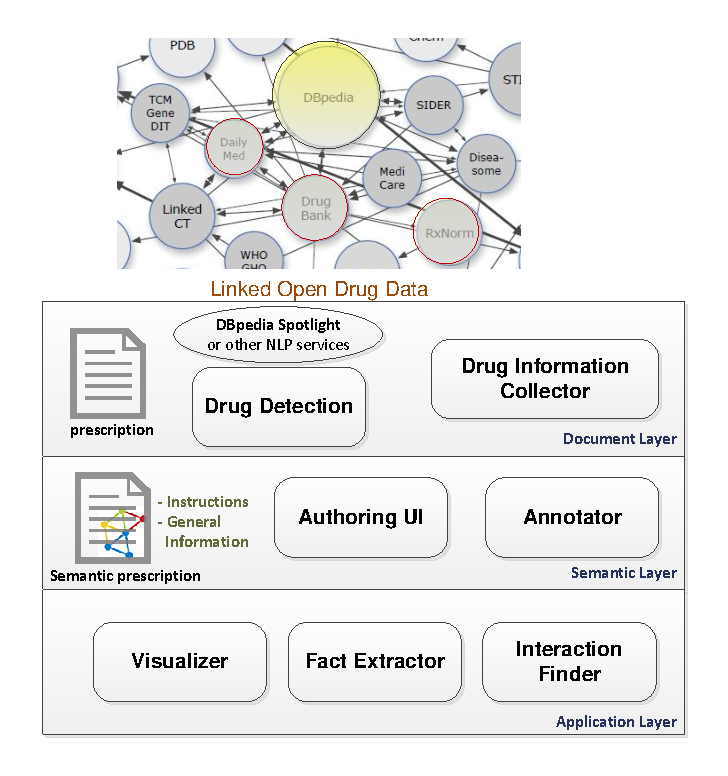
\includegraphics[width=1.0\columnwidth]{images/architecture.pdf}
	\caption{Architecture of the Pharmer system.}
	\label{fig:arch}
\end{figure}

\paragraph{Document Layer} This layer includes the traditional e-prescription document plus two components as \emph{Drug Detection} and \emph{Drug Information Collector}.
Drug detection component performs the natural language processing (NLP) of the e-prescription document to detect the terms referring to a drug in the prescription.
The component uses DBpedia spotlight\footnote{\url{http://spotlight.dbpedia.org/}} NLP service to parse and analyze the text looking for known drugs.
It is configurable so that users can easily add other existing NLP services for drug detection.
When user is writing the prescription, this component asynchronously performs the drug recognition and adds the related annotations as real-time semantic tagging.

Another component in this layer is drug information collector which grabs all the information regarding a specific drug from Linked Open Data.
To pursue this, it utilizes datasets such as DrugBank, DailyMed and RxNorm\footnote{Available at \url{http://www.w3.org/wiki/HCLSIG/LODD/Data}} by sending federated SPARQL\footnote{\url{http://www.w3.org/TR/rdf-sparql-query/}} queries.

\paragraph{Semantic Layer}
There are two main components in this layer namely \emph{Annotator} and \emph{Authoring UI}.
The \emph{annotator} component handles the automatic annotation and embeds the general information of the drugs as meta-data into the e-prescription.
Annotator adopts the RDFa format. \emph{RDFa}\footnote{\url{http://www.w3.org/TR/rdfa-syntax/}} (Resource Description Framework in attributes) is a W3C Recommendation that adds a set of attribute level extensions to XHTML for embedding RDF metadata within web documents.
RDFa fulfills the principles of interoperable metadata such as publisher independence, data reuse, self containment, schema modularity and evolvability to a good extent.

The \emph{authoring UI} component provides users with a set of input forms to manually embed the meta-data related to prescription instructions into the prescription document.

\paragraph{Application Layer}
This layer provides a set of applications on top of the generated semantic prescriptions.
\emph{Interaction Finder} checks the possible interactions between the prescribed drugs and warn the prescriber about them.
\emph{Visualizer} is responsible for graphically representing the embedded semantics of a prescription.
The \emph{Fact Extractor} generates the RDF/Turtle representation of the semantic prescriptions.


The Pharmer implementation is open-source and available for download together with an explanatory video and online demo\footnote{\url{http://bitili.com/pharmer}} at \url{http://code.google.com/p/pharmer/}.

\subsection{Features}
Drug Detection : DBpedia spotlight
Real-time semantic annotation
Interaction finder
Different views:
- Code View
- WYSIWYM
- Graph View
- Fact View

\begin{figure*}[tb]
	\centering
		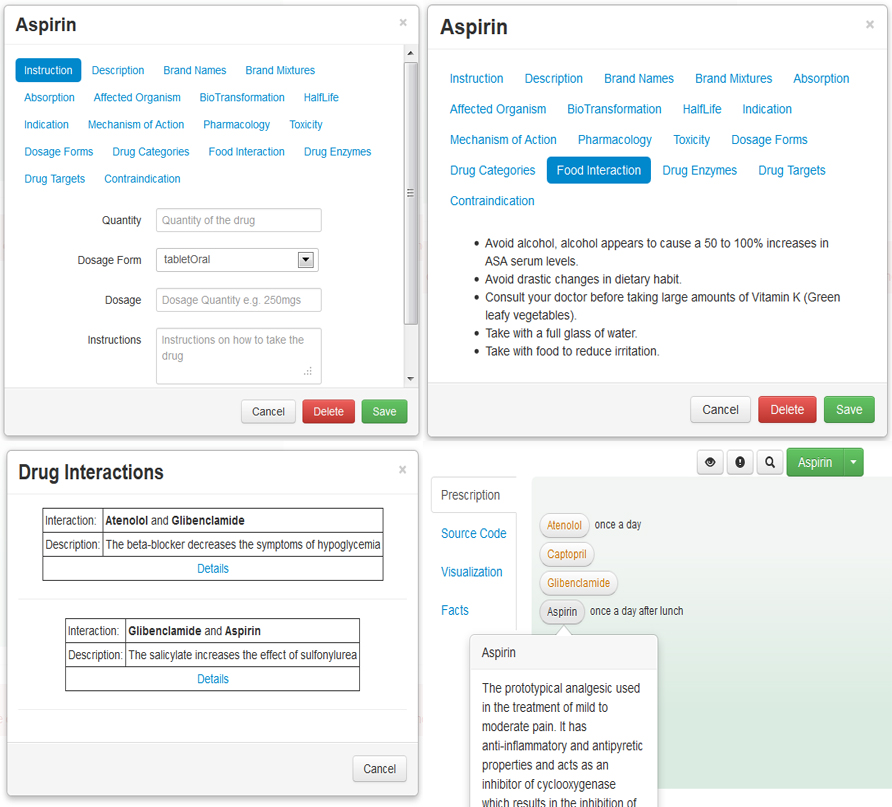
\includegraphics[width=2.0\columnwidth]{images/screenshot1.jpg}
	\caption{A screenshot of Pharmer information view.}
	\label{fig:wysiwym}
\end{figure*}

\begin{figure}[tb]
	\centering
		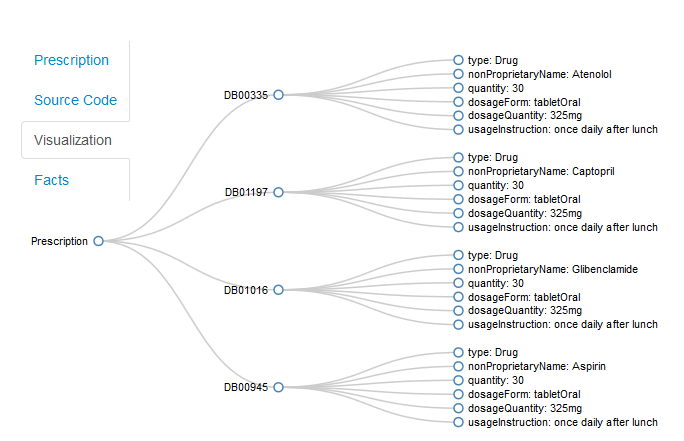
\includegraphics[width=1.0\columnwidth]{images/sc2.png}
	\caption{Graph View.}
	\label{fig:graphview}
\end{figure}



\section{Evaluation}
\label{evaluation}
In order to determine whether we succeeded to facilitate the creation of semantic prescriptions using Pharmer, we performed a usability user study with ? subjects.
Subjects were drawn from 3 physicians, 4 pharmacist, 10 pharmaceutical researchers and 5 students.
We first showed them a tutorial video of using different features of Pharmer then asked each one to create a prescription with Pharmer.
After finishing the task, we asked the participants to fill out a questionnaire which consisted of two parts: feature usage questions and usability experience questions.

We used the \emph{System Usability Scale} (SUS)~\cite{SUS2009} to grade the usability of Pharmer.
SUS is a standardized, simple, ten-item Likert scale-based questionnaire\footnote{\url{www.usabilitynet.org/trump/documents/Suschapt.doc}} giving a global view of subjective assessments of usability.
It yields a single number in the range of 0 to 100 which represents a composite measure of the overall usability of the system.
The results of our survey showed a mean usability score of ? for pharmer which indicates a reasonable level of usability.
Of course, this is a very simplified view on usability and we expect even better results could be achieved by putting more effort into the Pharmer development.
However, our goal was to demonstrate that Pharmer implementations with good usability characteristics can be created with relatively limited effort.
In addition to quantitative results, we also collected a number of user suggestions.
For instance some users suggested ?.


\section{Conclusion}
Improved confidentiality and security of health information, better clarity and communication among health care providers as well as rapid information exchange are part of arguments for spreading this system.

One of the most important advantages of E-prescribing is that the connection of physician, pharmacist, patient and pharmaceutical researchers and statision.
Once the E-prescription is written by a physician, pharmacist has also access to the prescription.
while the physician is aware, pharmacist can comment on the prescription content.
The online system is also available for patients who can inquire about any necessary information.
health care providers can follow up the patient's treatment fate.
The data base of the patients profile in subject of many statistics researches.
Besides, researchers are able to conveniently follow the drug in the clinical trial phase.

% conference papers do not normally have an appendix


% use section* for acknowledgement
\section*{Acknowledgment}


The authors would like to thank...
more thanks here

\bibliographystyle{IEEEtran}
% argument is your BibTeX string definitions and bibliography database(s)
\bibliography{sca_refs,refs}





% that's all folks
\end{document}


